\section{Methodology}
\label{sec:methodology}

\subsection{Problem Formulation and Backbone Architecture}
Let $\mathcal{U}$ be the set of users and $\mathcal{V} = \{1, 2, \dots, |\mathcal{V}|\}$ be the closed catalog of music tracks of size $|\mathcal{V}| = 98\,504$. A session for user $u \in \mathcal{U}$ is represented as an ordered sequence of track-duration pairs:
\begin{equation}
    \mathcal{S}_u = \big( (a_1, D_1), (a_2, D_2), \dots, (a_T, D_T) \big), \quad a_t \in \mathcal{V}, \; D_t \in \mathbb{R}^+,
\end{equation}
where $D_t$ denotes the continuous listening duration for track $a_t$ in seconds.

As our foundational architecture, we employ an autoregressive \textbf{Causal GPT-2} transformer~\cite{petrov2024aligning} initialized from scratch:
\begin{itemize}
    \item Vocabulary size: $|\mathcal{V}| + 1 = 98\,505$ (tokens $1 \dots 98\,504$ map to unique track IDs; index $0$ is reserved for \texttt{<PAD>}).
    \item Embedding dimension: $d_{\text{model}} = 384$.
    \item Attention blocks: $L = 3$, number of attention heads: $H = 4$.
    \item Context history window: $T_{\max} = 64$ tokens.
    \item Total parameters: \textbf{43\,174\,656} (~43.2M), all fully trainable.
\end{itemize}

The base model was trained on 33.2M interactions using mixed-precision FP16, AdamW optimizer ($\text{lr} = 10^{-3}$, $\text{weight\_decay} = 0.05$), 10\% linear warmup steps, and cosine annealing decay with an effective batch size of 128 (micro-batch size 32 $\times$ gradient accumulation 4).

\subsection{Reward Engineering and Formulation}
To incorporate consumption duration into the policy, we investigated three alternative scalar reward formulations $R(s, a)$ (Figure~\ref{fig:reward_formulations}):

\begin{figure}[!htbp]
    \centering
    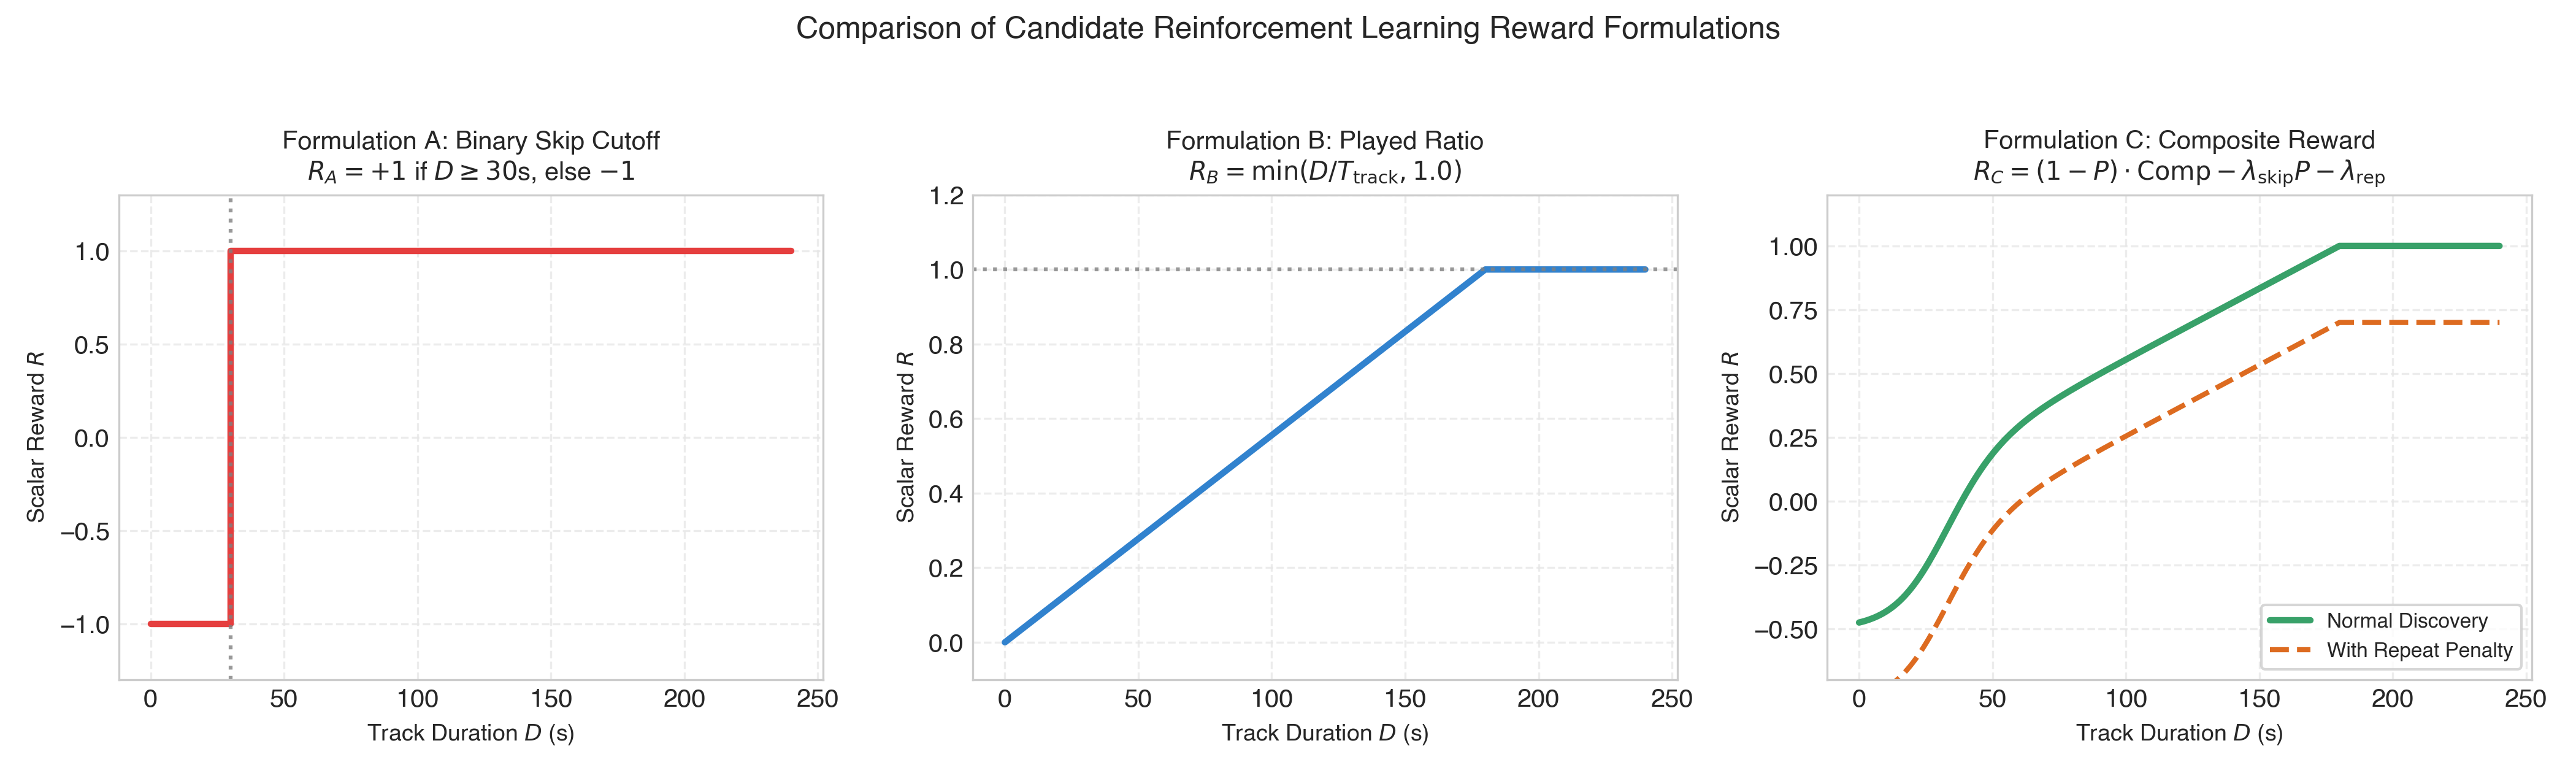
\includegraphics[width=0.86\textwidth]{fig2_reward_formulations_comparison.png}
    \caption{\textbf{Comparison of candidate reinforcement learning reward formulations.} A: Binary 30-second skip cutoff. B: Continuous played ratio normalized by track length. C: Multi-objective composite session reward with repetition penalty.}
    \label{fig:reward_formulations}
\end{figure}

\subsubsection{Formulation A: Binary Skip Cutoff}
The most robust signal separating successful plays from disliked skips:
\begin{equation}
    R_A(s, a) = \begin{cases} 
        +1.0, & \text{if } D(a) \ge 30\,\text{s}, \\ 
        -1.0, & \text{if } D(a) < 30\,\text{s}. 
    \end{cases}
    \label{eq:reward_a}
\end{equation}
The 30-second cutoff is the de-facto industrial standard: listens shorter than 30 seconds are unmonetized and unambiguously indicate user dissatisfaction.

\subsubsection{Formulation B: Continuous Played Ratio}
Normalizes listening duration $D(a)$ against the nominal duration of the track $T(a)$:
\begin{equation}
    R_B(s, a) = \min\left( \frac{D(a)}{T(a)}, 1.0 \right) \in [0.0, 1.0].
    \label{eq:reward_b}
\end{equation}
Preference pairs $(y_w \succ y_l)$ are mined by enforcing a minimum gap $\Delta R_B = R_B(y_w) - R_B(y_l) \ge 0.40$, which eliminates boundary noise.

\subsubsection{Formulation C: Multi-Objective Composite Reward}
Designed for Actor-Critic RL~\cite{matveev2026session}, combining skip probabilities, completion ratio, and an explicit penalty against immediate track repetition (\textit{Repeat Fatigue}):
\begin{equation}
    R_C(s, a) = \big(1 - P(\text{skip} \mid s, a)\big) \cdot \text{CompletionRatio}(s, a) - \lambda_{\text{skip}} P(\text{skip} \mid s, a) - \lambda_{\text{rep}} \mathbb{I}(a \in s_{t-3:t}),
    \label{eq:reward_c}
\end{equation}
where $\lambda_{\text{skip}} = 0.5$ and $\lambda_{\text{rep}} = 0.3$.

\subsection{Reinforcement Learning Alignment Paradigms}

\subsubsection{1. Two-Stage Critic Re-Ranking with $Q(s, a)$}
An independent state-action critic $Q_\phi(s, a)$ is trained to predict the expected reward $\mathbb{E}[R \mid s, a]$ on top of the frozen embeddings of the base transformer (two-layer MLP, 509K parameters)~\cite{petrov2024aligning}. At inference time, candidate items are scored via a linear combination of base logits and critic predictions:
\begin{equation}
    \text{Score}(a \mid s) = z_{\text{base}}(a \mid s) + \lambda \cdot Q_\phi(s, a), \quad \lambda \in \{0.1, 0.3, 0.5\}.
\end{equation}

To rigorously assess the Reward Model's performance on a held-out test split, Table~\ref{tab:critic_metrics} summarizes its empirical quality. While the Critic achieves a non-trivial ROC-AUC of 0.6120, its validation BCE loss stagnates at 0.5234, very close to the marginal Bernoulli entropy baseline $H(p=0.763) = 0.5488$ nats. Operating over frozen co-occurrence embeddings, the critic lacks raw acoustic signals, creating an expressive bottleneck that limits downstream reranking efficacy.

\begin{table}[!htbp]
\centering
\caption{\textbf{Held-out validation quality metrics of the State-Action Critic $Q_\phi(s, a)$ (509K params).} The Critic stagnates near the marginal Bernoulli entropy baseline, exhibiting the representation bottleneck of frozen embeddings.}
\label{tab:critic_metrics}
\vspace{0.3em}
\resizebox{\textwidth}{!}{%
\begin{tabular}{l ccccc}
\toprule
\textbf{Architecture / Model} & \textbf{Val BCE Loss} & \textbf{Bernoulli Entropy} & \textbf{Val ROC-AUC} & \textbf{Skip Acc.} & \textbf{Duration MAE} \\
\midrule
\textbf{Critic $Q_\phi(s, a)$ (2-layer MLP)} & \textbf{0.5234} & 0.5488 nats & \textbf{0.6120} & 76.1\% & 55.6s (baseline 56.4s) \\
\bottomrule
\end{tabular}%
}
\end{table}

\subsubsection{2. Actor-Critic PPO with KL Regularization}
The classic Proximal Policy Optimization framework~\cite{schulman2017proximal}. The actor generates distribution $\pi_\theta(a \mid s)$, and actions are sampled. To prevent policy collapse, the objective is regularized by Kullback--Leibler divergence with respect to the reference model:
\begin{equation}
    \max_\theta \mathbb{E}_{s \sim \mathcal{D}, a \sim \pi_\theta} \big[ R_C(s, a) \big] - \beta_{\text{KL}} \mathbb{D}_{\text{KL}}(\pi_\theta(\cdot \mid s) \parallel \pi_{\text{ref}}(\cdot \mid s)).
\end{equation}

\subsubsection{3. Direct Preference Optimization (DPO) with Auxiliary SFT Anchor}
Instead of fitting an unstable critic, DPO~\cite{rafailov2023direct} expresses the implicit reward function directly through the log-likelihood ratio of the active and reference policies:
\begin{equation}
    r(s, a) = \beta \log \frac{\pi_\theta(a \mid s)}{\pi_{\text{ref}}(a \mid s)}.
\end{equation}
Training is performed over preference triplets $\mathcal{D}_{\text{pref}} = \{(s, y_w, y_l)\}$, where $y_w$ is an engaged play ($D \ge 30$s) and $y_l$ is an immediate skip ($D < 30$s).

To prevent degradation of next-item likelihood, we introduce an \textbf{auxiliary SFT anchor}:
\begin{equation}
    \mathcal{L}_{\text{total}}(\theta) = \mathcal{L}_{\text{DPO}}(\theta; \pi_{\text{ref}}) + \gamma \cdot \mathcal{L}_{\text{SFT}}(y_w \mid s),
    \label{eq:dpo_sft}
\end{equation}
where
\begin{equation}
    \mathcal{L}_{\text{DPO}}(\theta; \pi_{\text{ref}}) = - \mathbb{E}_{(s, y_w, y_l) \sim \mathcal{D}_{\text{pref}}} \left[ \log \sigma \left( \beta \log \frac{\pi_\theta(y_w \mid s)}{\pi_{\text{ref}}(y_w \mid s)} - \beta \log \frac{\pi_\theta(y_l \mid s)}{\pi_{\text{ref}}(y_l \mid s)} \right) \right],
\end{equation}
and $\mathcal{L}_{\text{SFT}}(y_w \mid s) = - \log \pi_\theta(y_w \mid s)$ maximizes the likelihood of the preferred continuation.

\subsection{Evaluation Protocol and Statistical Testing}
Evaluation is conducted on a strictly held-out test split of \textbf{9,048 users} (\texttt{test\_interactions.parquet}) preserving full historical context. Item candidates are ranked across the \textbf{full catalog of 98,504 tracks} without negative sampling shortcuts.

Statistical reliability is verified through a rigorous testing suite:
\begin{enumerate}
    \item \textbf{Non-Parametric Bootstrap:} $B = 5\,000$ resamples with 95\% confidence intervals computed for HR@K, NDCG@K, MRR, and deltas $\Delta = \text{Metric}_{\text{DPO}} - \text{Metric}_{\text{Base}}$.
    \item \textbf{McNemar's Paired Test with Edwards' Continuity Correction:}
    \begin{equation}
        \chi^2 = \frac{(|n_{01} - n_{10}| - 1)^2}{n_{01} + n_{10}},
        \label{eq:mcnemar}
    \end{equation}
    where $n_{01}$ denotes users correctly recalled by DPO but missed by Base, and $n_{10}$ denotes the reverse.
    \item \textbf{Wilcoxon Signed-Rank Test:} Paired non-parametric test assessing distributional shift in individual ranking scores.
    \item \textbf{Catalog Health and Beyond-Accuracy Metrics:}
    \begin{itemize}
        \item \textit{Catalog Coverage \%:} Percentage of unique tracks recommended at least once in Top-10.
        \item \textit{Shannon Entropy:} $H = - \sum_{i=1}^{|\mathcal{V}|} p(i) \log_2 p(i)$, measuring distribution uniformity.
        \item \textit{Gini Coefficient:} Quantifying inequality across recommendation exposures.
        \item \textit{Spearman Rank Correlation with Popularity:} $\rho_s$, reflecting tendency to over-exploit head items.
    \end{itemize}
    \item \textbf{Autoregressive Queue Rollouts (Exposure Bias):} Simulating 5 consecutive unrolls ($s_t \to \hat{a}_{t+1} \to \dots \to \hat{a}_{t+5}$) without user feedback, measuring step-wise skip probabilities $P(\text{skip} \mid s_k, \hat{a}_k)$ and cumulative session play duration~\cite{matveev2026session}.
\end{enumerate}
